\clearpage
\section{Natural Systems} \label{Natural Systems}

    To create a bio-inspired control system for underwater locomotion, it is necessary to understand the basic morphology of fish and the physical properties of the water they manipulate to achieve their impressive agility. After understanding the structures and behaviors observed in  nature, they can be replicated in laboratory environments and applied to human designs. Drawing inspiration from a fish's mode of underwater sensing will present a method for closing the control loop in fish-inspired propulsion.

\subsection{Karman Vortex Streets} \label{Karman Vortex Streets}

    When fluids flow past bluff bodies, the bodies undergo a periodic cycle of forming and shedding low pressure regions on their downstream sides as the fluid imparts a drag force. These pressure regions consist of swirling fluid and are known as vortices. Each vortex circulates in the opposite direction of the previously shed vortex, and the wake of the bluff body becomes a line of oppositely rotating vortices shed from opposite sides of the body. This phenomenon was often observed, but it was little understood or studied before the publications from Theodore von Karman in 1911 \citep{Karman1911}. As such, the classic vortex wake formed by a smooth cylinder, shown in \Fref{fig:app:Karman}, is known as a Karman vortex street. For a bluff body, the vortex shedding frequency is related to a dimensionless parameter known as the Strouhal number 
    \begin{equation} \label{Eq:Karman St}
    St=\frac{fD}{U_\infty}
    \end{equation} 
    where \(f\) is the vortex shedding frequency, \(U_\infty\) is the free stream velocity, and \(D\) is the characteristic length of the body. In the case of a cylinder, \(D\) is the diameter. As the vortices rotate, the water between them forms jets with less momentum in the flow direction than the water upstream of the bluff body, which indicates a force imposed on the fluid by the body. In general, the force applied on a mass of water at two points in time is related by \[\int_{t_1}^{t_2} \vec F \, dt=m(\vec v_2-\vec v_1)\] where \(\vec F\) is the average force, \(t_1\) and \(t_2\) are the times at two moments, \(m\) is the mass of the water, and \(\vec v_1\) and \(\vec v_2\) are the fluid velocities at the two moments. By Newton's Third Law, the force applied on the water by a bluff body to create vortices is also applied on the bluff body by the water. The vortices, therefore, are a product of the force interaction between a bluff body and the surrounding fluid, and their characteristics vary based on the drag force imposed on the body.

\begin{figure}
\begin{center}
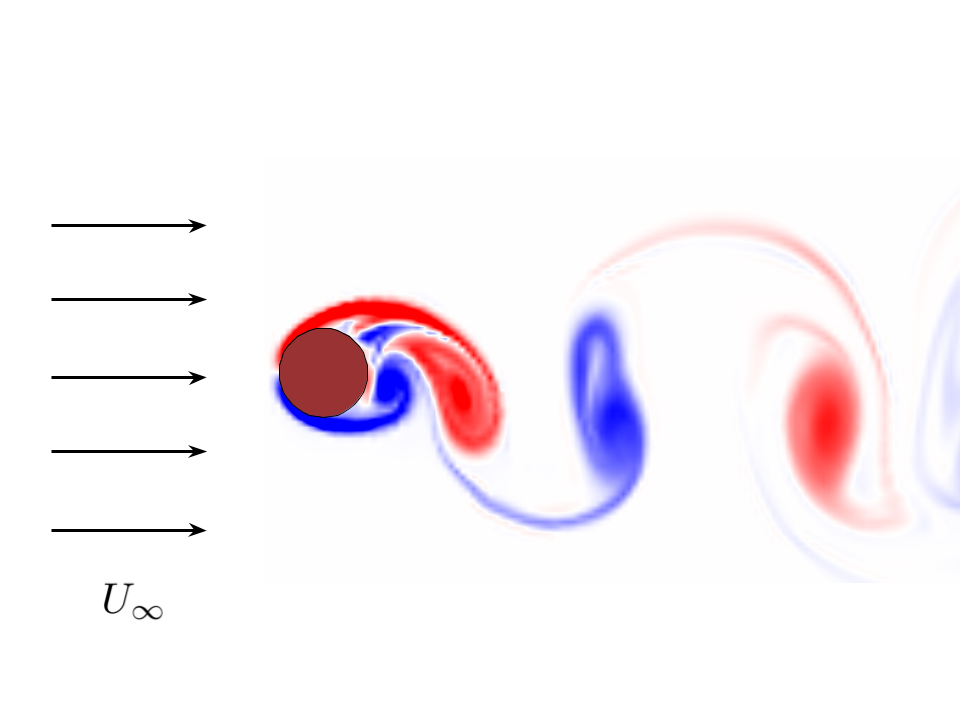
\includegraphics[width=0.6\columnwidth]{figures/Edited Karman Street.png}
\end{center}
\caption{Karman vortex street formed behind a circular cylinder in uniform flow, simulated in Lily Pad computational fluid dynamic (CFD) software \citep{Weymouth2015}. Arrows indicate the direction of free stream fluid flow, $U_\infty$. Red regions indicate clockwise flow, whereas blue regions indicate counterclockwise flow. Color intensity corresponds directly to the circulation intensity, also known as vorticity.}
\label{fig:app:Karman}
\end{figure}

\subsection{Fin Propulsion} \label{Fin Propulsion}

	 Beneath the surface of the water, organisms must contend with higher viscosity, larger drag forces, and often more prevalent predation than organisms that move through air. To overcome these challenges, marine animals, such as cartilaginous and bony fish, have developed the ability to use multiple control surfaces in tandem, enabling smaller turn radii and increased efficiency \citep{Bandyopadhyay2002,Lauder2004,Triant2020,Drucker2001}, which indicates improved agility. \Fref{fig:app:Bluegill} shows the basic fin placement of a ray finned fish using the well studied bluegill sunfish. \citep{Drucker2001} and \citep{Akhtar2007} observed that during forward propulsion ray finned fishes beat the water with their dorsal fins and caudal fins in a periodic motion consisting of two steps: heave and pitch. As \Fref{fig:app:Bluegill} illustrates, the pitch motion is the angular change in the fin’s orientation, while the heave motion is its lateral translation. The movement of a single fin is of the form 
\begin{equation} \label{Eq:Single foil heave}
Heave:  y(t)=Asin(2\pi f_h t)
\end{equation}
\begin{equation} \label{Eq:Single foil pitch}
Pitch: \theta (t)=\theta _msin(2\pi f_h t+\psi)
\end{equation}
    where \(y(t)\) is the position of the fin's leading edge, \(A\) is its amplitude, \(f_h\) is the flapping frequency in Hz, \(\theta(t)\) is the orientation of the fin relative to an inertial reference frame aligned with the incoming uniform flow, \(\theta _m\) is the maximum pitch, \(\psi\) is the phase shift between the two components of the fin motion, and \(t\) is the instantaneous time. During forward movement, the fins create vortex wakes that are nearly identical to those described in Section \ref{Karman Vortex Streets}, except the signs of the vortices are flipped. This street is known as a reverse Karman vortex street. The water momentum jet imposed by a standard Karman vortex street has less velocity in the flow direction, but in the reverse street, the velocity is higher. This is indicative of a thrust force, rather than a drag force. The Strouhal number describing this behavior becomes
    \begin{equation}\label{Eq:Fin St}
        St=\frac{2Af_h}{U_\infty}
    \end{equation}
    where the characteristic length, \(2A\), is the peak to peak amplitude of the oscillating fin. As generalized by \citep{Triant1993}, this  value ranges from 0.2-0.4 for nearly all animals that flap foils for propulsion, including insects, birds, bats, and fish, and this range is associated with the optimized energy input and thrust output. In the case of most bony fish, this value is near 0.25 for steady, forward propulsion \citep{Drucker2001, Nudds2014}.
    
\begin{figure}
\begin{center}
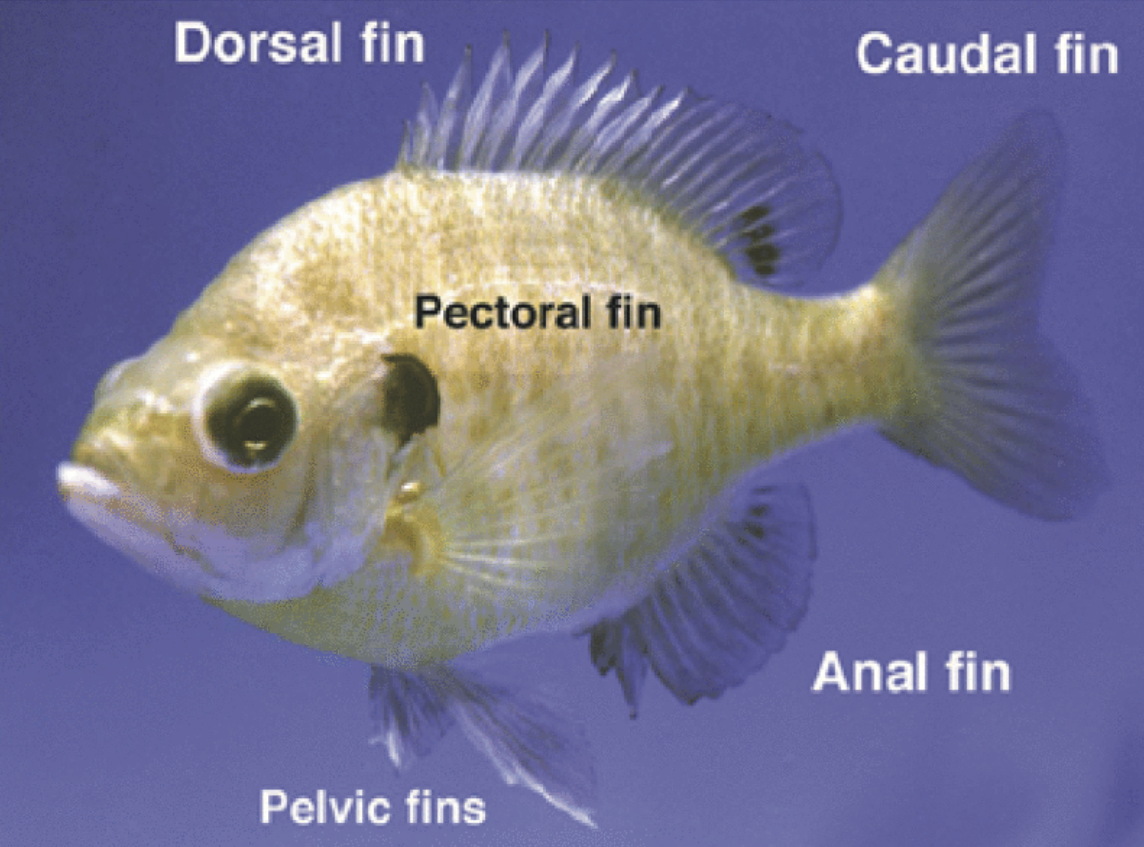
\includegraphics[width=0.44\columnwidth]{figures/Figure1.png}
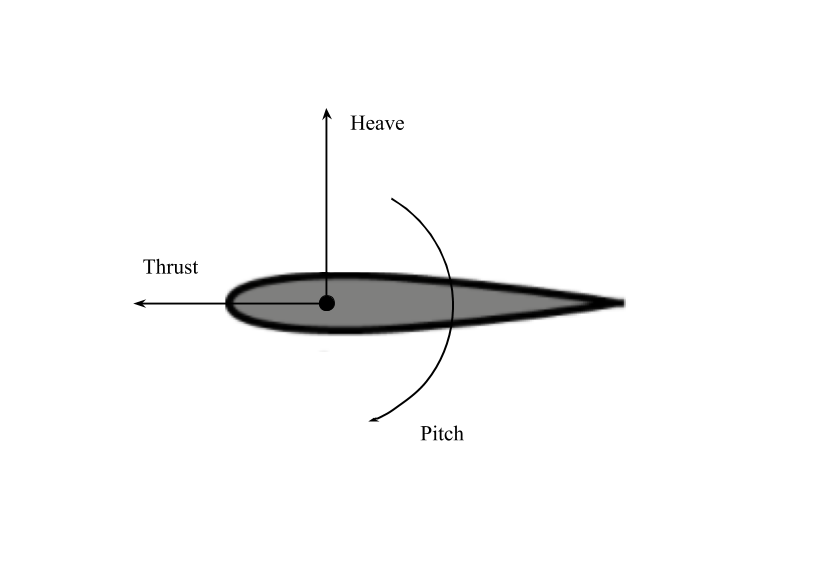
\includegraphics[width=0.54\columnwidth]{figures/Fin Frame.png}
\end{center}
\caption{Diagram of the fin arrangement on bluegill sunfish (left) \citep{Lauder2004}. Top-down view of a fin cross section with a superimposed coordinate grid (right).}
\label{fig:app:Bluegill}
\end{figure}

    During forward movement, the vortex street induced by the dorsal fin flows over the caudal fin, interfering with the caudal fin’s vortices \citep{Drucker2001, Akhtar2007}. This practice allows fish to change the effective angle of attack on their caudal fin and generate improved thrust, power, and efficiency. To reach these goals, the fins flap out of phase with one another \citep{Drucker2001}, and the phase difference causes the effective coefficient of thrust on the caudal fin to change, as shown in \Fref{fig:app:Fish Thrust}. This thrust coefficient, \(C_f\) is related to the fin's instantaneous thrust force by \[C_f=\frac{F}{0.5\rho U_\infty^2 A}\] where \(F\) is the thrust force, \(\rho\) is the water density, \(U_\infty\) is the free stream water velocity, and \(A\) is the fin surface area exposed to the flow. The dorsal fin moves according to (\ref{Eq:Single foil heave}) and (\ref{Eq:Single foil pitch}), while the caudal fin moves according to
    \begin{equation}
Heave: y_c(t)=A_csin(2\pi f_h t+\phi)
\end{equation}
\begin{equation} \label{Eq:Caudal fin pitch}
Pitch: \theta_c (t)=\theta _{mc}sin(2\pi f_h t+\psi+\phi)
\end{equation}
    where \(\phi\) represents the phase difference between the two fins, \(A_c\) represents the caudal fin's heave amplitude, and \(\theta_{mc}\) represents its maximum pitch angle. For bluegill sunfish and other ray finned fishes, \(A_c\) and \(\theta_{mc}\) are slightly greater than their dorsal counterparts \citep{Drucker2001}, although specific values vary depending on the fish species and behavior observed. The optimal \(\phi\) for a pair of tandem fins differs depending on anatomy and fin spacing. For the frequently studied bluegill sunfish shown in \Fref{fig:app:Bluegill}, maximum thrust is achieved at a phase difference of $\phi=48^o$, while other phase differences can achieve smaller increases or even decreases in thrust \citep{Akhtar2007}.

\begin{figure}
\begin{center}
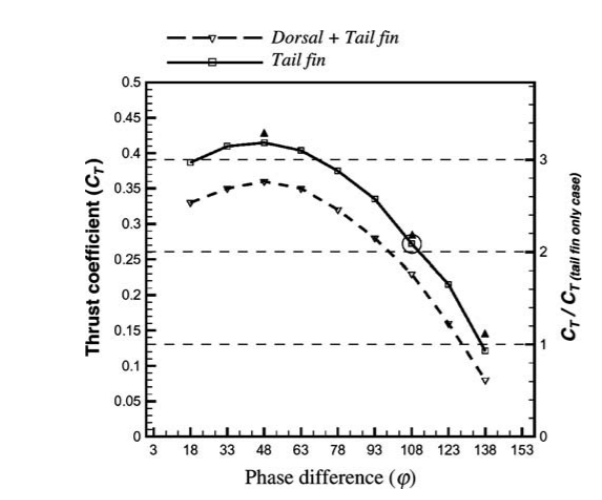
\includegraphics[width=0.49\columnwidth]{figures/Figure2.png}
\end{center}
\caption{Variation of caudal fin thrust coefficient with phase difference. The vertical axis is the thrust coefficient in absolute and normalized terms, while the phase difference is in degrees \citep{Akhtar2007}.}
\label{fig:app:Fish Thrust}
\end{figure}

\subsection{The Lateral Line Organ} \label{The Lateral Line Organ}

	Fish possess a unique sensory organ that allows them to detect both smooth and oscillating flow over their bodies: the lateral line. The line consists of a network of superficial and canal-embedded neuromasts, which deflect when fluid flows past them and stretch clusters of hair cells. These hair cells, in turn, trigger neurons to fire and transmit signals to the fish’s brain \citep{Dijkgraaf1962}. The general layout of the lateral line and the basic structure of the neuromasts are depicted in \Fref{fig:app:Lat Line}. The superficial neuromasts (SN) exist on the fish’s skin and protrude into the boundary layer. These sensors detect slow, steady changes in flow and have been characterized as velocity-sensitive \citep{Montgomery2001}. They typically detect flow changes that take place below 30 Hz \citep{Coombs2001}. The second group, the canal neuromasts (CN), exist as domed structures within small, fluid-filled canals that run beneath the surface of the fish’s skin. This canal is exposed to the outside flow through a series of pores. A CN perceives oscillating flow as pressure differences; when the pressure at one pore is different from the pressure at a pore farther down the canal, the canal fluid moves toward the pore of lower pressure, causing a deflection in the CN. When pressure changes slowly, typically below 30 Hz, the viscous forces within the canals prevent fluid movement \citep{Denton1989}, effectively acting as a high pass filter for pressure frequencies. Thus, CNs typically sense changes in flow that take place between 30 Hz and 150 Hz \citep{Coombs2001}. The pressure difference perceived by CNs can also be interpreted as a flow acceleration across the surface of the fish.
	
\begin{figure}
\begin{center}
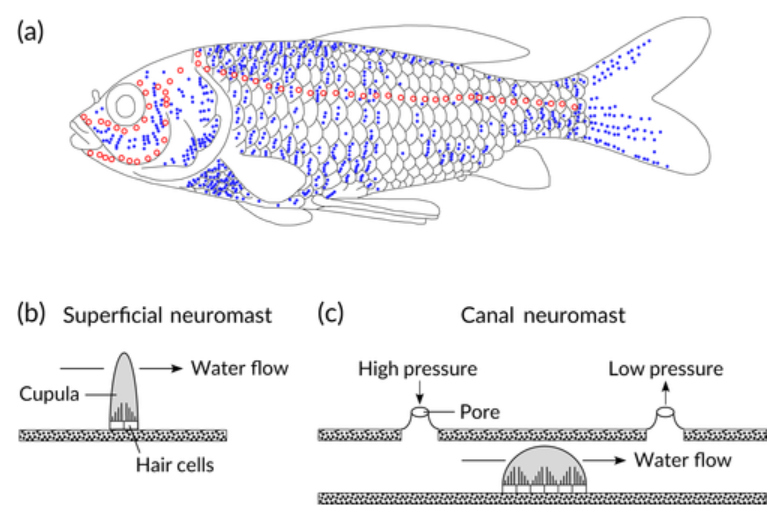
\includegraphics[width=0.49\columnwidth]{figures/Figure3.png}
\end{center}
\caption{(a) Basic anatomy of a lateral line in fish, where blue dots represent SNs and pink circles represent pores of the canal network. (b) Diagram of an SN. (c) Diagram of a CN \citep{Mogdans2018}.}
\label{fig:app:Lat Line}
\end{figure}

\subsubsection{Lateral Line Uses} \label{Lateral Line Uses}

	The lateral line allows fish to detect flow characteristics and collect information about their surroundings that are undetectable by visual or acoustic means. By detecting acute pressure and velocity changes, the lateral line enables fish to ‘feel’ objects that are several body lengths away, track prey by their wake \citep{Montgomery1995}, school with other fish, align with the local current \citep{Montgomery1999}, and adjust their gait for more efficient swimming in the presence of periodic flow \citep{Liao2003}. A particularly telling testimony to the effectiveness of lateral lines are the lifestyles of blind \citep{Windsor2010} and abyss-dwelling fish, which have been observed tracking prey and sensing obstacles with a spatial resolution of 1 mm \citep{Hassan1986}. The lateral line's ability to sense the presence of structures and flow characteristics without the fish's body coming in direct contact with them has come to be known as 'touch at a distance' \citep{Dijkgraaf1962}. 
	
	The lateral line enables fish to take advantage of wakes in the water to swim more efficiently. One such wake is the Karman vortex street, which is described in Section \ref{Karman Vortex Streets}. As \citep{Liao2003} observed, trout placed in a cylinder’s Karman vortex street detected the vortices’ positions and shedding frequency. The fish then adjusted their gaits to match the vortex shedding frequency and swam 180° out of phase with the vortex street, resulting in decreased muscle activity and, therefore, lower energy consumption. This behavior is depicted in a series of frames in \Fref{fig:app:Slalom}. Because the vortex wake was entirely invisible, the fish must have felt the flow characteristics and responded with a behavior that increased swimming efficiency \citep{Liao2003}.

\begin{figure}
\begin{center}
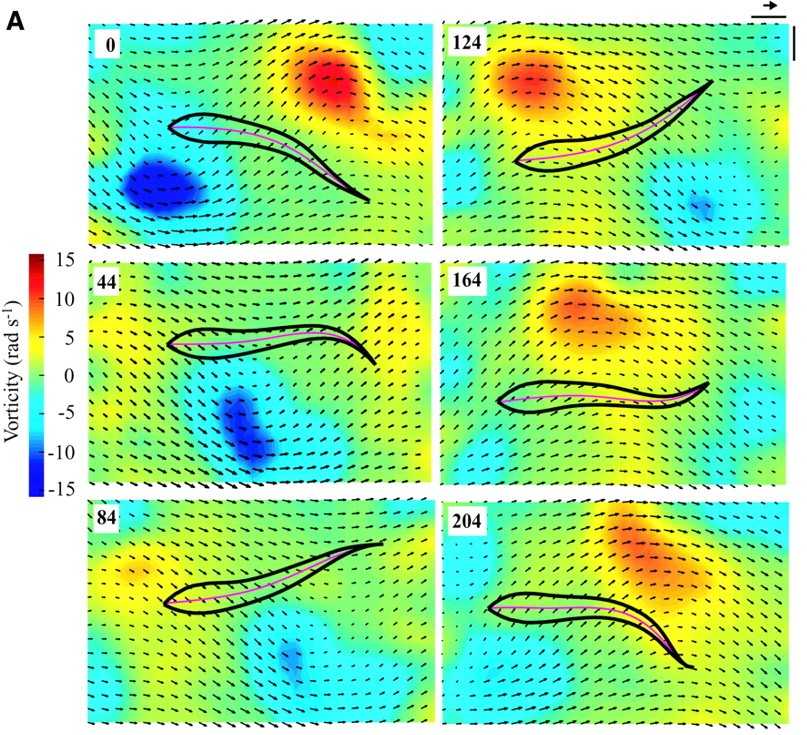
\includegraphics[width=0.49\columnwidth]{figures/Liao Slalom.jpg}
\end{center}
\caption{Bird's-eye view of a trout body outline slaloming through a Karman vortex street. The flow field was created with particle image velocimetry, and subplots are ordered sequentially proceeding from top to bottom on the left, then top to bottom on the right \citep{Liao2003}.}
\label{fig:app:Slalom}
\end{figure}

\subsection{Biological Inspiration}
    
    The slaloming behavior demonstrated by trout and the knowledge that fish fins induce similar vortices in their wake has spurred underwater robotics research to study and create control systems that utilize similar lateral line sensors to achieve more efficient or effective swimming in unmanned underwater vehicles (UUVs). Fish have already demonstrated that pressure-based control loops can be used to swim more effectively, and a lateral line sensing mechanism can provide the wake feedback necessary to develop effective tandem fin propulsion. The overarching theme of this project is to draw inspiration from the propulsion and wake sensing systems observed in nature to develop a control loop for an underwater propulsion system.